\documentclass[a4paper,11pt,uplatex]{jsarticle}


% 数式
\usepackage{amsmath,amsfonts}
\usepackage{bm}
\usepackage{physics}
% 画像
\usepackage[dvipdfmx]{graphicx}
\usepackage[dvipdfmx,colorlinks=true,linkcolor=blue]{hyperref}
\usepackage{pxjahyper}

\begin{document}


\section{結果}
\subsection{画像処理}
各ピクセルが持つ不定性の結果を示す。

\subsection{単アンジュレータ}
下流側のアンジュレータのみを用いて取得したデータの解析結果を示す。
このデータを用いてパラメータの較正をおこなった。

\subsubsection{放射光および光学系パラメータ}
回折パターンの形状を決定するパラメータはアンジュレータ - スリット間距離、スリット - カメラ間距離、スリット幅の3つである。
これに加えて放射光関数の情報も形状を決定する。

\subsubsection{距離依存性}
アンジュレータと光学系の距離に依存して光量が変化する。
立体角を考えるとこの光量は距離rに対して$\frac{1}{r^2}$に比例する

\subsection{振動パターン}
2つのアンジュレータの放射光による干渉パターンの振動を解析する。


\subsection{系統誤差}
\subsubsection{波長依存性}
異なる波長でエネルギーを決定する

\subsubsection{距離依存性}
下流側アンジュレータの位置を4つの区間に分割し、各区間でエネルギーを決定した。
これによりフィット関数が持つ位置依存性による系統誤差を見積もることができる。

\subsubsection{エネルギー依存性}
180.195,210 MeVの3つのエネルギーの結果












\clearpage

\begin{figure}[tb]
  \centering
  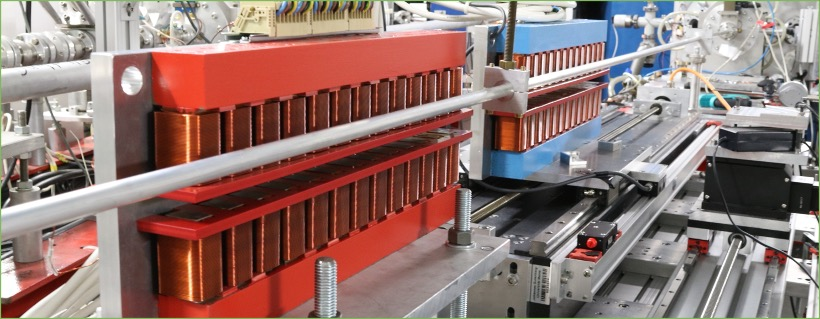
\includegraphics[width=0.8\linewidth]{image/1-1.jpg}\\
  \caption{サンプルの図}
  \label{sample_image}
\end{figure}

\begin{itemize}
  \item a
\end{itemize}
\begin{enumerate}
  \item b
\end{enumerate}

\begin{align}
\frac{1}{2} = \qty(\frac{1}{3}) + \qty{1}\Sigma
\end{align}
\end{document}